\section{Кинематика вращательного движения материальной точки}

\introProblems

\begin{ex} %Сив43
Луна обращается вокруг Земли с периодом $T = 27,3$ сут относительно звезд. Средний радиус орбиты Луны $R = 3,8 \cdot 10^5$ км. Найти линейную скорость $v$ движения Луны вокруг Земли и ее нормальное ускорение $a$. 
\begin{ans}
$v = 2 \pi R/T = 3,7$ км/ч; $a = 4\pi^2 R/T^2 = 35$ км/ч\textsuperscript{2}.
\end{ans}
\end{ex}

\begin{ex} %Сив54
Якорь электромотора, вращавшегося с частотой $N$ оборотов в секунду, двигаясь после выключения тока равнозамедленно, остановился, сделав $n$ оборотов. Найти угловое ускорение якоря после выключения тока.
\begin{ans}
$\varepsilon = \pi N^2/n$.
\end{ans}
\end{ex}

\begin{ex} %Сив58
Автомобиль, движущийся со скоростью 40 км/ч, проходит закругление шоссе с радиусом кривизны 200 м. На повороте шофер тормозит машину, сообщая ей ускорение 0,3 м/с\textsuperscript{2}. Найти нормальное и полное ускорение автомобиля на повороте. Как направлен вектор полного ускорения $\vec{a}$ по отношению к радиусу кривизны $R$ закругления шоссе?
\begin{ans}
$a_n = 0.6$ м/с\textsuperscript{2}; $a = 0.67$ м/с\textsuperscript{2}; угол между векторами $\vec{a}$ и $\vec{R}$ составляет $135^{\circ}$.
\end{ans}
\end{ex}

\begin{ex} %Сив62
Колесо радиуса $R$ равномерно катится без скольжения по горизонтальному пути со скоростью $v$. Найти координаты $x$ и $y$ произвольной точки $A$ на ободе колеса, выразив их как функции времени $t$ или угла поворота колеса $\varphi$, полагая, что при $t = 0$ $\varphi = 0$, $x = 0$, $y = 0$ (рис. \ref{cycloid}). По найденным выражениям для $x$ и $y$ построить график траектории точки на ободе колеса.

\begin{figure}[h]
\centering
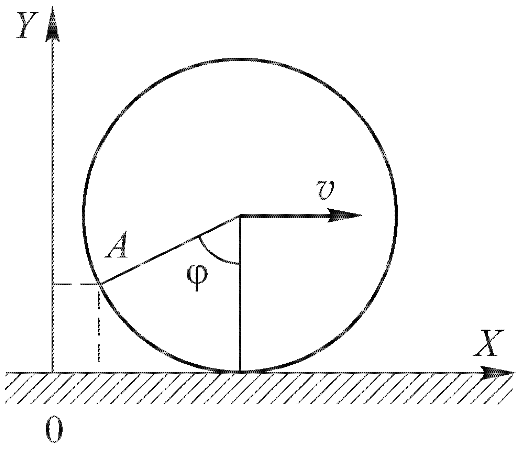
\includegraphics[width=0.3\textwidth]{cycloid.png}
\caption{}
\label{cycloid}
\end{figure}

\begin{ans}
$x= R(\varphi - \sin \varphi) = R(\omega t - \sin \omega t)$, $y=R(1-\cos \varphi) = R(1-\cos \omega t)$, где $\omega = v/R$ -- угловая скорость вращения колеса. Траекторией точек, находящихся на ободе движущегося колеса, будет простая циклоида.
\end{ans}
\end{ex}

\qualProblems

\begin{ex} %Сив44
Каковы будут графики зависимости от времени абсолютных величин скорости и ускорения при равномерном движении точки по кругу?
\end{ex}

\begin{ex}
Точка $A$ движется со скоростью 1 м/с, а точка $B$ – со скоростью 2 м/с, причем скорости этих точек
сонаправлены. Может ли расстояние $AB$ оставаться неизменным?
\end{ex}

\begin{ex}
Луна постоянно обращена к Земле одной стороной. Сколько оборотов совершит она вокруг своей оси за время полного оборота вокруг Земли?
\end{ex}

\begin{ex}
Будет ли происходить смена дня и ночи на Земле, если она перестанет вращаться вокруг своей оси?
\end{ex}

\begin{ex} 
Во сколько раз угловая скорость часовой стрелки больше угловой скорости суточного вращения Земли?
\end{ex}

\begin{ex} 
Ускорения двух материальных точек, движущихся по окружностям одного и того же радиуса, равны по модулю. Однако ускорение первой точки направлено под углом $45^{\circ}$ к касательной, а ускорение второй – по радиусу. У какой из этих точек больше скорость?
\end{ex}

\begin{ex} 
Почему верхние спицы катящегося колеса велосипеда иногда сливаются в одно целое, в то время как нижние видны раздельно?
\end{ex}

\begin{ex} 
Сплошной диск катится без проскальзывания по горизонтальному участку пути с постоянной скоростью. Какие точки диска имеют относительно неподвижного наблюдателя такую же по модулю скорость, что и центр диска?
\end{ex}

\begin{ex} %Сив42
Точка движется равномерно по плоской траектории, изображенной на рис. \ref{maxAccel}. В каком месте траектории ускорение точки будет максимальным?

\begin{figure}[h]
\centering
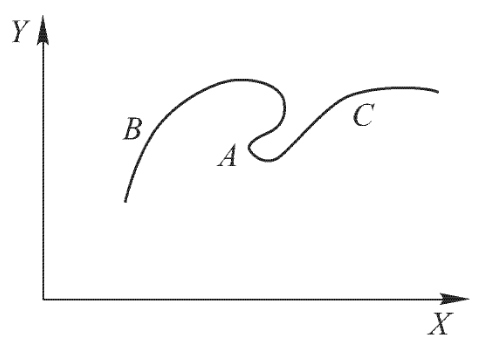
\includegraphics[width=0.4\textwidth]{maxAccel.png}
\caption{}
\label{maxAccel}
\end{figure}
\begin{ans}
A.
\end{ans}
\end{ex}

\begin{ex} %Сив44
Математический маятник отклонили на угол $\alpha = 45^{\circ}$ от положения равновесия и отпустили без начальной скорости. Под каким углом к горизонту направлен вектор ускорения маятника в начальный момент времени?
\begin{ans}
$90^{\circ}$.
\end{ans}
\end{ex}

\begin{ex}
Какую линию составляют концы векторов скорости материальной точки, равномерно вращающейся по окружности, если все векторы, соответствующие скорости снаряда в каждый момент времени, построить из одной точки. Искомый график называется годографом вектора скорости.
\end{ex}

\begin{ex}
Жесткий стержень скользит в вертикальной плоскости, опираясь своими концами на пол и стену. По какой траектории движется середина стержня?
\end{ex}

\simpleProblems

\begin{ex} %Сив45
Найти среднюю угловую скорость искусственного спутника Земли, если период обращения его по орбите вокруг Земли составляет 105 мин.
\begin{ans}
$\omega \approx 0.001$ c\textsuperscript{-1}.
\end{ans}
\end{ex}

\begin{ex} %Сив49
Найти линейную скорость Земли, вызванную ее орбитальным движением. Средний радиус земной орбиты равен $R = 1.5 \cdot 10^8$ км.
\begin{ans}
$v \approx 30$ км/с.
\end{ans}
\end{ex}

\begin{ex} %Сив55
Автомобиль движется со скоростью 60 км/ч. Сколько оборотов в секунду делают его колеса, если они катятся по шоссе без скольжения, а внешний диаметр покрышек колес равен 60 см.
\begin{ans}
$\nu \approx 9$ об/с.
\end{ans}
\end{ex}

\begin{ex} %Сив57
Разматывая веревку и вращая без скольжения вал ворота, ведро опускается в колодец с ускорением 1 м/с\textsuperscript{2}. С каким угловым ускорением вращается вал ворота? Как зависит от времени угол поворота вала? Радиус вала ворота равен 25 см.
\begin{ans}
$\varepsilon = 4$ рад/c\textsuperscript{2}; $\varphi = 2t^2$ рад.
\end{ans}
\end{ex}

\begin{ex} %Чертов1.56
Маховик начал вращаться равноускоренно с за промежуток времени $t=10$ с достиг частоты вращения $n=300$ об/мин. Определите угловое ускорение $\varepsilon$ маховика и число оборотов $N$, которое он сделал за это время.
\begin{ans}
$\varepsilon =  3.14$ рад/\textsuperscript{2}, $N = 25$.
\end{ans}
\end{ex}

\begin{ex} %Чертов1.49
Тело брошено под углом $\alpha = 30^{\circ}$ к горизонту. Найти тангенциальное и нормальное ускорения в начальный момент движения.
\begin{ans}
5 м/c\textsuperscript{2}, 8.7 м/c\textsuperscript{2}.
\end{ans}
\end{ex}

\begin{ex} %Сив66
Представление о величине и направлении вектора полного ускорения при ускоренном вращательном движении (например, для точек якоря электромотора при его пуске) можно получить, рассмотрев следующую задачу. Точка движется по окружности радиусом $R$ с постоянным тангенциальным ускорением $a_{\tau}$, но без начальной скорости. Найти нормальное и полное ускорения точки, выразив их: 1) как функцию от времени $t$ и ускорения $a_{\tau}$; 2) как функцию от углового ускорения $\varepsilon$ и угла поворота $\varphi$ радиуса-вектора точки из его начального положения. Найти угол $\beta$ между направлением вектора полного ускорения точки и ее
радиусом-вектором.
\begin{ans}
$a_n = \frac{a_{\tau}^2 t^2}{R} = 2 \varepsilon R \varphi$; $a = \frac{a_{\tau}}{R} \sqrt{R^2 + a_{\tau}^2 t^4} = \varepsilon R \sqrt{1 + 4 \varphi^2}$; $\tg \beta = -\frac{1}{2\varphi}$.
\end{ans}
\end{ex}

\complexProblems

\begin{ex} %Сив59
Колесо радиуса $R$ катится без скольжения по горизонтальной дороге со скоростью $v_0$ (рис. \ref{rollingWheel}). Найти горизонтальную компоненту $v_x$ линейной скорости движения произвольной точки на ободе колеса, вертикальную компоненту $v_y$ этой скорости и модуль полной скорости для этой же точки. Найти значение угла $\alpha$ между вектором полной скорости точек на ободе колеса и направлением поступательного движения его оси. Показать, что направление вектора полной скорости произвольной точки $A$ на ободе колеса всегда перпендикулярно к прямой $AB$ и проходит через высшую точку катящегося колеса. Показать, что для точки $A$: $v = BA \omega$. Построить график распределения скоростей для всех точек на вертикальном диаметре (в данный момент времени) катящегося без скольжения колеса. Выразить все искомые величины через $v_0$, $R$ и угол $\varphi$, составленный верхним вертикальным радиусом колеса и радиусом, проведенным из центра колеса $O$ в исследуемую точку его обода $A$.

\begin{figure}[h]
\centering
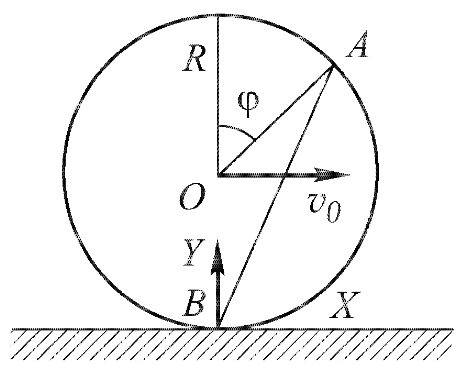
\includegraphics[width=0.4\textwidth]{rollingWheel.png}
\caption{}
\label{rollingWheel}
\end{figure}

\begin{ans}
$v_x = v_0 (1 + \cos \varphi) = 2v_0 \cos^2 \frac{\varphi}{2}$; $v_y = -v_0 \sin \varphi$; $v = 2v_0 \cos \frac{\varphi}{2}$.
\end{ans}
\end{ex}

\begin{ex} %Сив64
Автомобиль с колесами радиуса $R$ движется со скоростью $v$ по горизонтальной дороге, причем $v^2 > Rg$, где $g$ -- ускорение свободного падения. На какую максимальную высоту $H_{\max}$ может быть заброшена вверх грязь, срывающаяся с колес автомобиля? Указать положение той точки на покрышке колеса, с которой при данной скорости движения автомобиля грязь будет забрасываться выше всего. Сопротивление воздуха движению отброшенной вверх грязи не учитывать.
\begin{ans}
$H_{\max} = R + \frac{v^2}{2g} + \frac{gR^2}{2v^2}$; $\cos \varphi^{*} = - \frac{Rg}{v^2}$.
\end{ans}
\end{ex}

\begin{ex} %Иродов1.57

\begin{figure}[h]
\centering
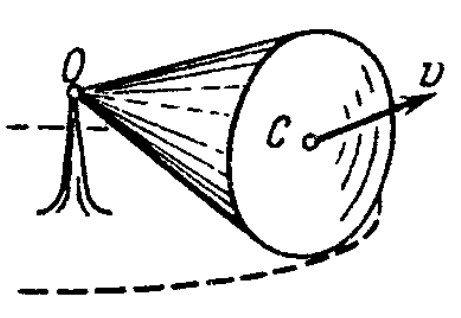
\includegraphics[width=0.4\textwidth]{rollingCylinder.png}
\caption{}
\label{rollingCylinder}
\end{figure}

Круглый конус с углом полураствора $\alpha = 30^{\circ}$ и радиусом основания $R = 5,0$ см катится равномерно без скольжения по горизонтальной плоскости, как показано на рис. \ref{rollingCylinder}. Вершина конуса закреплена шарнирно в точке $O$, которая находится на одном уровне с точкой $C$ -- центром основания конуса. Скорость точки $C$ равна $v = 10,0$ см/с. Найти модули: 1) угловой скорости конуса; 2) углового ускорения конуса.

\begin{ans}
1) $\omega = \frac{v}{R \cos \alpha} = 0,6$ рад/с; 2) $\varepsilon = (v/R)^2 \tg \alpha = 2,3$ рад/c\textsuperscript{2}.
\end{ans}
\end{ex}

\clearpage